
%{{第六十四回}}{第六十四回}}

\chapter{幽淑女悲题五美吟 浪荡子情遗九龙佩}

{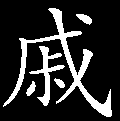
\includegraphics[width=3mm]{../Images/00005} \kaishu 此一回紧接贾敬灵柩进城,原当铺叙宁府丧仪之盛,但上回秦氏病故,凤姐理丧,已描写殆尽,若仍极力写去,不过加倍热闹而已。故书中于迎灵送殡极忙乱处,却只闲闲数笔带过。忽插入钗玉评诗、琏尤赠佩一段闲雅{[}风流{]}文字来,正所谓``急脉缓受''也。}

题曰:

深闺有奇女,绝世空珠翠。情痴苦泪多,未惜颜憔悴。

哀哉千秋魂,薄命无二致。嗟彼桑间人,好丑非其类。

话说贾蓉见家中诸事已妥,连忙赶至寺中,回明贾珍。于是连夜分派各项执事人役,并预备一切应用幡杠等物。择于初四日卯时请灵柩进城,一面使人知会诸位亲友。

是日,丧仪炫耀,宾客如云,自铁槛寺至宁府,夹路而观者,何啻万数。也有羡慕的,也有嗟叹的。又有一等半瓶醋的读书人,说是``丧礼与其奢易莫若俭戚''的,一路纷纷议论不一。至未申时方到,将灵柩停放正室之内。供奠举哀已毕,亲友渐次散回,只剩族中人分理迎宾送客等事。近亲只有邢大舅等未去。贾珍贾蓉此时为礼法所拘,不免在灵旁藉草枕苫\href{../Text/part0068_split_000.html\#lnkback_1_a}{\textsuperscript{①}},恨苦居丧。人散后,仍乘空寻他小姨厮混。宝玉亦每日在宁府穿孝,至晚人散,方回园里。凤姐身体未愈,虽不能时常在此,或遇开坛诵经、亲友上祭之日,亦扎挣过来,相帮尤氏料理料理。

一日,供毕早饭,因此时天气尚长,贾珍等连日劳倦,不免在灵旁假寐。宝玉见无客至,遂欲回家看视黛玉,因先回至怡红院中。进入门来,只见院中寂静,悄无人声,有几个老婆子与小丫头们在回廊下取便乘凉,也有睡卧的,也有坐着打盹的。宝玉也不去惊动。只有四儿看见,连忙上前来打帘子。将掀起时,只见芳官自内带笑跑出,几乎与宝玉撞个满怀。一见宝玉,方含笑站住,说道:``你怎么来了?你快与我拦住晴雯,他要打我呢。''一语未了,只听得屋内咭溜咕噜的乱响,不知是何物撒了一地。随后晴雯赶来骂道:``我看你这小蹄子往那里去!输了不叫打。宝玉又不在家,我看谁来救你!''宝玉连忙拦住,笑道:``你妹子小,不知怎么得罪了你,看我的分上饶他罢。''晴雯也不想宝玉此时回来,乍一见,不觉好笑,遂笑说道:``芳官竟是狐狸精变的,就是会拘神遣将的,符咒也没有这样快。''又笑道:``就是你真请了神来,我也不怕。''遂夺手仍要捉拿芳官。芳官早已藏在宝玉身后。

宝玉遂一手拖了晴雯,一手携了芳官,进入屋内。看时,只见西边炕上麝月、秋纹、碧痕、紫绡等正在那里抓子儿赢瓜子呢。却是芳官输与晴雯,芳官不肯叫打,跑了出去。晴雯因赶芳官,将怀内的子儿撒了一地。宝玉欢喜道:``如此长天,我不在家,正恐你们寂寞,吃了饭睡觉,睡出病来,大家寻件事顽笑消遣甚好。''因不见袭人,又问道:``你袭人姐姐呢?''晴雯道:``袭人么?越发道学了,独自一个在屋里面壁呢。这好一会我们没进去,不知他作什么呢,一些声气也听不见。你快瞧瞧去罢,或者此时参悟了也未可定。''

宝玉听说,一面笑,一面走至里间。只见袭人坐在近窗的床上,手中拿着一根灰色绦子,正在那里打结子呢。见宝玉进来,连忙站起,笑道:``晴雯这东西编派我什么呢?我因要赶着打完这结子,没工夫和他们瞎闹,因哄他们道:`你们玩去罢,趁着二爷不在家,我要在这里静坐一坐,养一养神。'他就编派了许多混话,什么`面壁了'`参禅了'的,等一会我不撕他那嘴!''

宝玉笑着挨近袭人坐下,瞧他打结子,问道:``这么长天,你也该歇息歇息,或和他们玩去,要不,瞧瞧林妹妹去也好。怪热的,打这个那里使?''袭人道:``我见你带的扇套还是那年东府里蓉大奶奶的事情上做的。那个青东西除族中或亲友家夏天有丧事方带得着,一年遇着带一两遭,平常又不犯做。如今那府里有事,这是要过去天天带的,所以我赶着另作一个。等打完了结子,给你换下那旧的来。你虽然不讲究这个,若叫老太太回来看见,又该说我们躲懒,连你穿带之物都不经心了。''宝玉笑道:``这真难为你想得到。只是也不可过于赶,热着了,倒是大事。''说着,芳官早托了一杯凉水内新湃的茶来。因宝玉素昔秉赋柔脆,虽\elegantpar{暑月不敢用冰}{应是有冰库},只以新汲井水将茶连壶浸在盆内,不时更换,取其凉意而已。宝玉就芳官手内吃了半盏,遂向袭人道:``我来时已吩咐了茗烟,若珍大哥那边有要紧人客来时,令彼即来通禀;若无甚要事,我就不过去了。''说毕,遂出了房门,又回头向碧痕等道:``如有事,往林姑娘处来找我。''于是一径往潇湘馆来看黛玉。

将走过沁芳桥,只见雪雁领着两个老婆子,手中都拿着菱藕瓜果之类。宝玉忙问雪雁道:``你们姑娘从来不大吃这些凉东西的,拿这些瓜果何用?莫非是要请那位姑娘、奶奶么?''雪雁笑道:``我告诉你,可不许你对姑娘说去。''宝玉点头应允。雪雁便命两个婆子:``先将瓜果送去交与紫鹃姐姐。他要问我,你就说我做什么呢,就来。''那婆子答应着去了。雪雁方说道:``我们姑娘这两日方觉身上好些了。今日饭后,三姑娘来,会着要瞧二奶奶去,姑娘也没去。又不知想起甚么来,自己伤感了一会,题笔写了好些,不知是诗啊词啊。叫我传瓜果去时,又听叫紫鹃将屋内摆着的小琴桌上的陈设搬下来,将桌子挪在外间当地,又叫将那龙文鼒{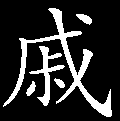
\includegraphics[width=3mm]{../Images/00005}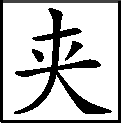
\includegraphics[width=3mm]{../Images/00012}\footnotesize \kaishu 子之切,小鼎也。}放在桌上,等瓜果来时听用。若说是请人呢,不犯先忙着把个炉摆出来;若说点香呢,我们姑娘素日屋内除摆新鲜花儿、木瓜、佛手之类,又不大喜熏香;就是点香,亦当点在常坐卧之处。难道是老婆子们把屋子熏臭了,要拿香熏熏不成?究竟连我也不知何故。''说毕,便连忙去了。

宝玉这里,不由得低头细想,心内道:``据雪雁说来,必有原故。若是同那一位姊妹们闲坐,亦不必如此先设馔具。或者是姑爹、姑妈的忌辰,但我记得每年到此日期,老太太都吩咐另外整理肴馔,送去与林妹妹私祭,此时已过。大约是因七月为瓜果之节,家家都上秋祭的坟,林妹妹有感于心,所以在私室自己奠祭,取《礼记》`春秋荐其时食'之意,也未可定。但我此刻走去,见林妹妹伤感,必极力劝解,又怕他烦恼郁结于心;若竟不去,又恐他过于伤感,无人劝止;两件皆足致疾。莫若先到凤姐姐处一看,在彼稍坐即回。如若见林妹妹伤感,再设法开解,既不至使其过悲,哀痛稍申,亦不至抑郁致病。''\elegantpar{想毕}{思虑深远},遂出了园门,一径到凤姐处来。

正有许多执事婆子们回事毕,纷纷散出。凤姐儿正倚着门和平儿说话呢。一见了宝玉,笑道:``你回来了么?我才吩咐了林之孝家的,叫他使人告诉跟你的小厮,若没什么事,趁便请你回来歇息歇息。再者那里人多,你那里禁得住那些气味。不想恰好你倒来了。''宝玉笑道:``多谢姐姐记挂。我也因今日没事,又见姐姐这两日没往那府里去,不知身上可大愈否,所以回来看视看视。''凤姐道:``左右也不过是这样,三日好两日不好的。老太太、太太不在家,这些大娘们,嗳,那一个是安分的!每日不是打架,就拌嘴,连赌博偷盗的事情都闹出来了两三件了。虽说有三姑娘帮着办理,他又是个没出阁的姑娘。\elegantpar{也有好叫他知道的,也有对他说不得的事,也只好强扎挣着罢了。}{大约贾蓉是晓得的}总不得心静一会。别说想病好,求其不添也就罢了。''宝玉道:``虽如此说,姐姐还要保重身体,少操些心才是。''说毕,又说了些闲话,别过凤姐,一直往园中走来。

进了潇湘馆的院门看时,只见炉袅残烟,奠馀玉醴。紫鹃正看着人往里搬桌子,收陈设呢。宝玉便知已经祭完了,走入屋内,只见黛玉面向里歪着,病体恹恹,大有不胜之态。紫鹃连忙说道:``宝二爷来了。''黛玉方慢慢的起来,含笑让坐。宝玉道:``妹妹这两天可大好些了?气色倒觉静些,只是为何又伤心了?''黛玉道:``可是你没的说了,好好的我多早晚又伤心了?''宝玉笑道:``妹妹脸上现有哭泣之状,如何还哄我呢。只是我想妹妹素日本来多病,凡事当各自宽解,不可过作无益之悲。若作践坏了身子,将来使我\ldots{}\ldots{}''说到这里,觉得以下的话有些难说,连忙咽住。只因他虽说和黛玉自小一处长大,情投意合,又愿同生死,却只是心中领会,从来未曾当面说出。况兼黛玉心重,每每因说话造次,得罪了他,致彼哭泣。今日原为的是来劝解黛玉,不想把话来说造次了,接不下去,心中一急,又怕黛玉恼他。又想一想自己的心实在是为好,因而转急为悲,早已滚下泪来。黛玉起先原恼宝玉说话不论轻重,如今见此光景,心有所感,本来素昔爱哭,此时亦不免\elegantpar{无言对泣}{难怪贾母操碎了心}。

却说紫鹃端了茶来,打量他二人不知又为何事角口,因说道:``姑娘才身上好些,宝二爷又来怄气来了,到底是怎么样?''宝玉一面拭泪,笑道:``谁敢怄妹妹了!''一面搭讪着起来闲步。只见砚台底下微露一纸角,不禁伸手拿起。黛玉忙要起身来夺,已被宝玉揣在怀内,笑央道:``好妹妹!赏我看看罢。''黛玉道:``不管什么,来了就混翻。''

一语未了,只见宝钗走来,笑道:``宝兄弟要看什么?''宝玉因未见上面是何言词,又不知黛玉心中如何,未敢造次回答,却望着黛玉笑。黛玉一面让宝钗坐,一面笑说道:``我曾见古史中有才色的女子,终身遭际,令人可喜、可羡、可悲、可叹者甚多。今日饭后无事,因择出数人,胡乱凑几首诗,以寄感慨。可巧探丫头来会我瞧凤姐姐去,我因身上懒懒的,没同他去。适才做了五首,一时困倦起来,撂在那里,不想二爷来了,就瞧见了。其实给他看也倒没有什么,但只我嫌他是不是的写了给人看去。''宝玉忙道:``我多早晚给人看来呢?昨日那把扇子,原是我爱那几首白海棠的诗,所以我自己用小楷写了,不过为的是拿在手中看着便易。\elegantpar{我岂不知闺阁中诗词字迹是轻易往外传诵不得的?}{见宝钗来了也只是笑。}自从你说了,我总没拿出园子去。''宝钗道:``林妹妹这虑得也是。你既写在扇子上,偶然忘记了,拿在书房里去,被相公们看见了,岂有不问是谁做的呢。倘或传扬开了,反为不美。自古道`女子无才便是德',总以贞静为主,女工还是第二件。其馀诗词之类,不过是闺中游戏,原可以会,可以不会。咱们这样人家的姑娘,倒不要这些才华的名誉。''因又笑向黛玉道:``拿出来给我看看无妨,只不叫宝兄弟拿出去就是了。''黛玉笑道:``既如此说,连你也可以不必看了。''又指着宝玉笑道:``他早已抢了去了。''宝玉听了,方自怀内取出,凑至宝钗身旁,一同细看。只见写道:

西 施

一代倾城逐浪花,吴宫空自忆儿家。

效颦莫笑东村女,头白溪边尚浣纱。

虞 姬

肠断乌骓夜啸风,虞兮幽恨对重瞳。

黥彭甘受他年醢,饮剑何如楚帐中!

昭 君\href{../Text/part0068_split_000.html\#lnkback_2_a}{\textsuperscript{②}}

绝艳惊人出汉宫,红颜薄命古今同。

君王纵使轻颜色,予夺权何畀画工?

绿 珠

瓦砾明珠一例抛,何曾石尉重娇娆!

都缘顽福前生造,更有同归慰寂寥。

红 拂

长揖雄谈态自殊,美人巨眼识穷途。

尸居馀气杨公幕,岂得羁縻\elegantpar{女丈夫}{好}!

宝玉看了,赞不绝口,又说道:``妹妹这诗,恰好只做了五首,何不就命名曰《五美吟》。''于是不容分说,便提笔写在后面。{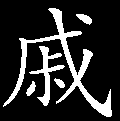
\includegraphics[width=3mm]{../Images/00005}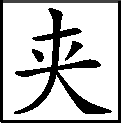
\includegraphics[width=3mm]{../Images/00012}\footnotesize \kaishu 《五美吟》与后《十独吟》对照。}宝钗亦说道:``做诗不论何题,只要善翻古人之意。若要随人脚踪走去,纵使字句精工,已落第二义,究竟算不得好诗。即如前人所咏昭君之诗甚多,有悲挽昭君的,有怨恨延寿的,又有讥汉帝不能使画工图貌贤臣而画美人的,纷纷不一。后来王荆公复有`意态由来画不成,当时枉杀毛延寿';永叔有`耳目所见尚如此,万里安能制夷狄'。二诗俱能各出己见,不袭前人。今日林妹妹这五首诗,亦可谓命意新奇,别开生面了。''

仍欲往下说时,只见有人回道:``琏二爷回来了。适才外间传说,往东府里去了好一会了,想必就回来的。''宝玉听了,连忙起身,迎至大门以内等待。恰好贾琏自外下马进来。于是宝玉先迎着贾琏跪下,口中给贾母、王夫人等请了安,又给贾琏请了安。二人携手走了进来。只见李纨、凤姐、宝钗、黛玉、迎、探、惜等早在中堂等候,一一相见已毕。因听贾琏说道:``老太太明日一早到家,一路身体甚好。今日先打发了我来回家看视,明日五更,仍要出城迎接。''说毕,众人又问了些路途的景况。因贾琏是远路适归,遂大家别过,让贾琏回房歇息。一宿晚景,不必细述。

至次日饭时前后,果见贾母、王夫人等到来。众人接见已毕,略坐了一坐,吃了一杯茶,便领了王夫人等人过宁府中来。只听见里面哭声震天,却是贾赦、贾政\href{../Text/part0068_split_000.html\#lnkback_3_a}{\textsuperscript{③}}送贾母到家,即过这边来了。当下贾母进入里面,早有贾赦、贾政率领族中人哭着迎了出来。赦、政一边一个挽了贾母,走至灵前,又有贾珍、贾蓉跪着,扑入贾母怀中痛哭。贾母暮年人,见此光景,亦搂了珍、蓉等痛哭不已。贾赦、贾政在旁苦劝,方略略止住。又转至灵右,见了尤氏婆媳,不免又相持大痛一场。哭毕,众人方上前一一请安问好。贾珍因贾母才回家来,未得歇息,坐在此间看着,未免要伤心,遂再三求贾母回家,王夫人等亦再三相劝。贾母不得已,方回来了。

果然,年迈的人禁不住风霜伤感,至夜间,便觉头闷身酸,鼻塞声重。连忙请了医生来诊脉下药,足足的忙乱了半夜一日。幸而发散得快,未曾传经,至三更天,些须发了点汗,脉静身凉,大家方放了心。至次日仍服药调理。又过了数日,乃贾敬送殡之期,贾母犹未大愈,遂留宝玉在家侍奉。凤姐因未曾甚好,亦未去。其馀贾赦、贾政、邢夫人、王夫人等率领家人仆妇,都送至铁槛寺,至晚方回。贾珍、尤氏并贾蓉仍在寺中守灵,等过百日后,方扶柩回籍。家中仍托尤老娘并二姐、三姐照管。

却说贾琏素日既闻尤氏姐妹之名,恨无缘得见。近因贾敬停灵在家,每日与二姐、三姐相识已熟,不禁动了垂涎之意。况知与贾珍、贾蓉等素有\elegantpar{聚麀之诮}{是新词了},因而乘机百般撩拨,眉目传情。那三姐却只是淡淡相对,只有二姐也十分有意,但只是眼目众多,无从下手。贾琏又怕贾珍吃醋,不敢轻动,只好二人心领神会而已。此时出殡以后,贾珍家下人少,除尤老娘带领二姐、三姐并几个粗使的丫鬟、老婆子在正室居住外,其馀婢妾都随在寺中。外面仆妇,不过晚间巡更,日间看守门户,白日无事,亦不进里面去。所以贾琏便欲趁此下手,遂托相伴贾珍为名,亦在寺中住宿,又时常借着替贾珍料理家务,不时至宁府中来勾搭二姐。

一日,有小管家俞禄来回贾珍道:``前者所用棚杠孝布并请杠人青衣,共使银一千两,除给银五百两外,仍欠五百两。昨日两处买卖人俱来催讨,奴才特来讨爷的示下。''贾珍道:``你向库上去领就是了,这又何必来问我。''俞禄道:``昨日已曾向库上去领,但只是老爷宾天以后,各处支领甚多,所剩还要预备百日道场及庙寺中用度,此时竟不能发给。所以奴才今日特来回爷,或者爷内库里暂且发给,或者挪借何项,吩咐了奴才好办。''贾珍笑道:``\elegantpar{你还当是先呢,有银子放着不使。}{现在是亏空起来了。}你无论那里暂且借了给他罢。''俞禄笑回道:``若说一二百,还可以巴结,这四五百两,一时那里办得来!''贾珍想了一想,向贾蓉道:``你问你娘去,昨日出殡以后,有江南甄家送来打祭银五百两,未曾交到库上去,你先要了来,给他去罢。''贾蓉答应了,连忙过这边来,回了尤氏,复转来回他父亲道:``昨日那项银子已使了二百两,下剩的三百两,令人送至家中,交与老娘收了。''贾珍道:``既然如此,你就带了他去,向你老娘要了出来交给他。再也瞧瞧家中有事无事,问你两个姨娘好。下剩的,俞禄先借了添上罢。''

贾蓉与俞禄答应了,方欲退出,只见贾琏走了进来。俞禄忙上前请了安。贾琏便问何事,贾珍一一告诉了。贾琏心中想道:``趁此机会,正可至宁府寻二姐。''一面遂说道:``这有多大事,何必向人借去。昨日我方得了一项银子,还没有使呢,莫若给他添上,岂不省事?''贾珍道:``如此甚好。你就吩咐了蓉儿,一并令他取去。''贾琏忙道:``这必得我亲身取去。再我这几日没回家了,还要给老太太、老爷、太太们请请安去。再到阿哥那边查查家人们有无生事,也给亲家太太请请安。''贾珍笑道:``只是又劳动你老二,我心不安。''贾琏也笑道:``自家兄弟,这又何妨。''贾珍又吩咐贾蓉道:``你跟了你叔叔去,也到那边给老太太、老爷、太太们请安,说我和你娘都请安,打听打听老太太身上可大安了,还服药呢没有?''贾蓉一一答应了,跟随贾琏出来,带了几个小厮,骑上马,一同进城。

在路叔侄闲话。贾琏有心,便提到尤二姐,因夸说如何标致,如何做人好,举止大方,言语温柔,无一处不令人可敬可爱,``人人都说你婶子好,据我看那里及你二姨一零儿呢。''贾蓉揣知其意,便笑道:``叔叔既这么爱他,我给叔叔作媒,说了做二房何如?''贾琏笑道:``敢是好呢。只怕你婶子不依,再也怕你老娘不愿意。况且我听见说,你二姨已有了人家了。''贾蓉道:``这都无妨。我二姨、三姨都不是我老爷养的,原是我老娘带了来的。听见说我老娘在那一家时,就把我二姨许给皇庄张家,指腹为婚。后来张家遭了官司,败落了,我老娘又自那家嫁了出来,如今这十数年,两家音信不通。我老娘时常抱怨,要与他家退婚,我父亲也要将二姨转聘。只等有了好人家,不过令人找着张家,给他数两银子,写上一张退婚的字儿。想张家穷极了的人,见了银子,有什么不依的。再他也知道咱们这样的人家,也不怕他不依。又是叔叔这样人说了做二房,我管保我老娘和我父亲都愿意。倒只是婶子那里却难。''

贾琏听到这里,心花都开了,那里还有什么话说,只是一味呆笑而已。贾蓉又想了一想,笑道:``叔叔若有胆量,依我的主意行去,管保无妨,不过多花上几个钱。''贾琏忙道:``有何主意,快些说来,我没有不依的。''贾蓉道:``叔叔回家,一点声色也别露。等我回明了我父亲,向我老娘说妥,然后在咱府后方近左右,买上一所房子及应用家伙什物,再拨两窝子家下人过去伏侍。择了日子,人不知,鬼不觉,娶了过去,嘱咐家人不许走漏风声。嫂子在里面住着,深宅大院,那里就得知道了。叔叔两下里住着,过个一年半载,即或闹出来,不过挨上老爷一顿骂。叔叔只说婶子总不生育,原是为子嗣起见,所以私自在外面作成此事。就是婶子,见生米做成熟饭,也只得罢了。\elegantpar{再求一求老太太,没有不完的事}{国舅老爷总有护身符}。''

自古道``欲令智昏'',贾琏只顾贪图二姐美色,听了贾蓉一篇话,遂为计出万全,将现今身上有服,并停妻再娶,严父妒妻种种不妥之处,皆置之度外了。却不知贾蓉亦非好意,素日因同他两个姨娘有情,只因贾珍在内,不能畅意。如今若是贾琏娶了,少不得在外居住,趁贾琏不在时,好去鬼混之意。贾琏那里意想及此,遂向贾蓉致谢道:``好侄儿,你果然能够说成了,我买两个绝色的丫头谢你。''说着,已至宁府门首。贾蓉说道:``叔叔进去,向我老娘要出银子来,就交给俞禄罢。我先给老太太请安去。''贾琏含笑点头道:``老太太跟前,别提我和你一同来的。''贾蓉道:``知道。''又附耳向贾琏道:``今日要遇见二姨,可别性急了,闹出事来,往后倒难办了。''贾琏笑道:``少胡说!你快去罢。我在这里等你。''于是贾蓉自去给贾母请安。

贾琏进入宁府,早有家人头儿率领家人等请安,一路围随至厅上。贾琏一一的问了些话,不过塞责而已,便命家人散去,独自往里面走来。

原来贾琏、贾珍素日亲密,又是弟兄,本无可避忌之人,自来是不等通报的。于是走至上房,早有廊下伺候的老婆子打起帘子,让贾琏进去。贾琏进入房中一看,只见南边炕上只有尤二姐带着两个丫鬟一处做活,却不见尤老娘与三姐。贾琏忙上前问好相见。尤二姐亦含笑让坐,贾琏便靠东边板壁坐了,仍将上首让与二姐,寒温毕,贾琏笑问道:``亲家太太和三妹妹那里去了。怎么不见?''尤二姐笑道:``才有事往后头去了,也就来的。''此时,伺候的丫鬟因倒茶去,无人在跟前,贾琏便睨视二姐一笑。二姐亦低了头,只含笑不理。贾琏又不敢造次动手动脚,因见二姐手中拿着一条拴着荷包的手巾摆弄,便搭讪着往腰内摸了摸,说道:``槟榔荷包也忘记带了来,妹妹有槟榔,赏我一口吃。''二姐道:``槟榔倒有,只是我的槟榔从来不给人吃。''

贾琏便笑着,欲近身来拿。二姐怕人看见不雅,便连忙一笑,撂了过来。贾琏接在手中,都倒了出来,\elegantpar{拣了半块吃剩下的,撂在口中吃了}{吃槟榔},又将剩下的都揣了起来。刚要把荷包亲身送过去,只见两个丫鬟倒了茶来。贾琏一面接了茶吃茶,一面暗将自己带的一个汉玉九龙佩解了下来,拴在手绢上,趁丫鬟回头时,仍撂了过去。二姐亦不去拿,只装看不见,仍坐着吃茶。只听后面一阵帘子响,却是尤老娘、三姐带着两个小丫头自后面走来。贾琏送目与二姐,令其拾取,这尤二姐亦只是不理。贾琏不知二姐何意,甚是着急,只得迎上来与尤老娘、三姐相见。一面又回头看二姐时,只见二姐笑着,没事人似的,再又看一看手巾,已不知那里去了,贾琏方放了心。

于是大家归坐后,叙了些闲话。贾琏说道:``大嫂子说,前日有一包银子交给亲家太太收起来了,今日因要还人,大哥令我来取。再也看看家里有事无事。''尤老娘听了,连忙使二姐拿钥匙去取银子。这里贾琏又说道:``我也要给亲家太太请请安,瞧瞧二位妹妹。亲家太太脸面倒好,只是二位妹妹在我们家里受委屈。''尤老娘笑道:``咱们都是至亲骨肉,说那里的话。在家里也是住着,在这里也是住着。不瞒二爷说,我们家里自从先夫去世,家计也着实艰难了,全亏了这里姑爷帮助。如今姑爷家里有了这样大事,我们不能别的出力,白看一看家还有什么委屈了的呢。''正说着,二姐已取了银子来,交与尤老娘。尤老娘便递与贾琏。贾琏叫一个小丫头叫了一个老婆子来,吩咐他道:``你把这个交给俞禄,叫他拿过那边去等我。''老婆子答应了出去。

只听得院内是贾蓉的声音说话。须臾进来,给他老娘、姨娘请了安,又向贾琏笑道:``才刚老爷还问叔叔呢,说是有什么事情要使唤。原要使人到寺里去叫,我回老爷说,叔叔就来。老爷还吩咐我,路上遇着叔叔叫快去呢。''贾琏听了,忙要起身,又听贾蓉和他老娘说道:``那一次我和老太太说的,我父亲要给二姨说的姨爹,就和我这叔叔的面貌身量差不多儿。老太太说好不好?''一面说着,又悄悄的用手指着贾琏,和他二姨努嘴。二姐倒不好意思说什么,只见三姐笑骂道:``坏透了的小猴儿崽子!没了你娘的说了,等我撕他那嘴!''一面说着,便赶了过来。贾蓉早笑着跑了出去,贾琏也笑着辞了出来。走至厅上,又吩咐了家人们不可耍钱吃酒等话;又悄悄的央贾蓉,回去急速和他父亲说。一面便带了俞禄过来,将银子添足,交给他拿去;一面自己见他父亲,给贾母去请安,不提。

却说贾蓉见俞禄跟了贾琏去取银子,自己无事,便仍回至里面,和他两个姨娘嘲戏一回,方起身。至晚到寺,见了贾珍,回道:``银子已经交给俞禄了。老太太已大愈了,如今已经不服药了。''说毕,又趁便将路上贾琏要娶尤二姐做二房之意说了。又说如何在外面置房子住,不使凤姐知道,``此时总不过为的是子嗣艰难起见,为的是二姨是见过的,亲上做亲,比别处不知道的人家说了来的好。所以二叔再三央我对父亲说。''\elegantpar{只不说是他自己的主意}{叔侄一路货色}。

贾珍想了想,笑道:``其实倒也罢了。只不知你二姨心中愿意不愿意。明日你先去和你老娘商量,叫你老娘问准了你二姨,再作定夺。''于是又教了贾蓉一篇话,便走过来,将此事告诉了尤氏。尤氏却知此事不妥,因而极力劝止。无奈贾珍主意已定,素日又是顺从惯了的,况且他与二姐本非一母,不便深管,因而也只得由他们闹去了。

至次日一早,果然贾蓉复进城来见他老娘,将他父亲之意说了,又添上许多话,说贾琏做人如何好,目今凤姐身子有病,已是不能好的了,暂且买了房子,在外住着,过个一年半载,只等凤姐一死,便接了二姨进去做正室。又说他父亲此时如何聘,贾琏那边如何娶,如何接了你老人家养老,往后三姨也是那边应了替聘,说得天花乱坠,不由得尤老娘不肯。况且素日全亏贾珍周济,此时又是贾珍作主替聘,一切妆奁不用自己置买,贾琏又是年轻公子,比张华胜强十倍,遂连忙过来合二姐商议。二姐又是水性的人,在先已合姐夫不妥,又时常怨恨当时错许张华,使后来终身失所,今见贾琏有情,况且是姐夫将他聘嫁,有何不肯,亦便点头应允。当下回复了贾蓉,贾蓉回了他父亲。

次日,便请了贾琏到寺中来,贾珍当面告诉了他尤老娘应允之事。贾琏自是喜出望外,又感谢贾珍、贾蓉父子不尽。于是三人商议,使人看房子、打首饰,给二姐置买妆奁及新房中应用床帐等物。不多几日,早将诸事办妥。已于宁荣街后二里远近小花枝巷内买定一所房子,共二十馀间。又买了几个小丫头。贾珍又给了一房家人,叫鲍二夫妻两口,以备二姐过去时伏侍。又使人将张华父子找来,逼着与尤老娘写了退婚书。

且说张华之祖,原当皇庄,后来死了。至张华父亲时,仍充此役,因与尤老娘前夫相好,所以将张华与二姐指腹为婚。后来不料遭了官司,败落家产,弄得衣食不周,那里还娶得媳妇。尤老娘又自那家嫁了出来,两家有十数年音信不通。今被贾府家人唤来,逼他与二姐退婚,心中虽不愿意,无奈惧怕贾珍等势力,不敢不依,只得写了一张退婚文约。尤老娘与银十两家去,不提。

这里贾琏见诸事已妥,遂择了初三黄道吉日,娶二姐过门。未知如何,下回分解。正是:

只为同枝贪色欲,致教连理起戈矛。

{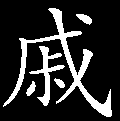
\includegraphics[width=3mm]{../Images/00005}\kaishu 总评:五首新诗何所居,颦儿应自日欷}歔{。柔肠一段千般结,岂是寻常望雁鱼。}

{\kaishu 五百年风流债,一见了偏作怪。你贪我爱自难休,天巧姻缘浑无奈。}

{\kaishu 父母者于子女间,莫失教训说前缘。防微之处休弛纵,严厉才能真爱怜。}

% {\href{../Text/part0068_split_000.html\#navto_1_a}{①}``藉草枕苫'',各本皆同。按《仪礼·既夕礼》贾公彦疏有``寝以苫,以块枕头''语,故程本改``苫''为``块''。}

% {\href{../Text/part0068_split_000.html\#navto_2_a}{②}``昭君'',除底本外,馀本均作``明妃''。}

% {\href{../Text/part0068_split_000.html\#navto_3_a}{③}贾政之名本回共出现五次(蒙、杨、甲辰本,列本因一句错夺少了一次)。按,因列、杨本没有第三十七回贾政点学差的情节,此时贾政出现在理丧现场并不矛盾。但诸本是有贾政点学差的情节的,故戚本对人名作了改易,但不彻底,只改了前面四处。到了程本才全部改掉。}
